
\documentclass[tikz, border=10pt]{standalone}
\usepackage{tikz}
\usetikzlibrary{positioning, chains, shapes.geometric, fit, shapes, arrows.meta, calc, backgrounds}

\begin{document}
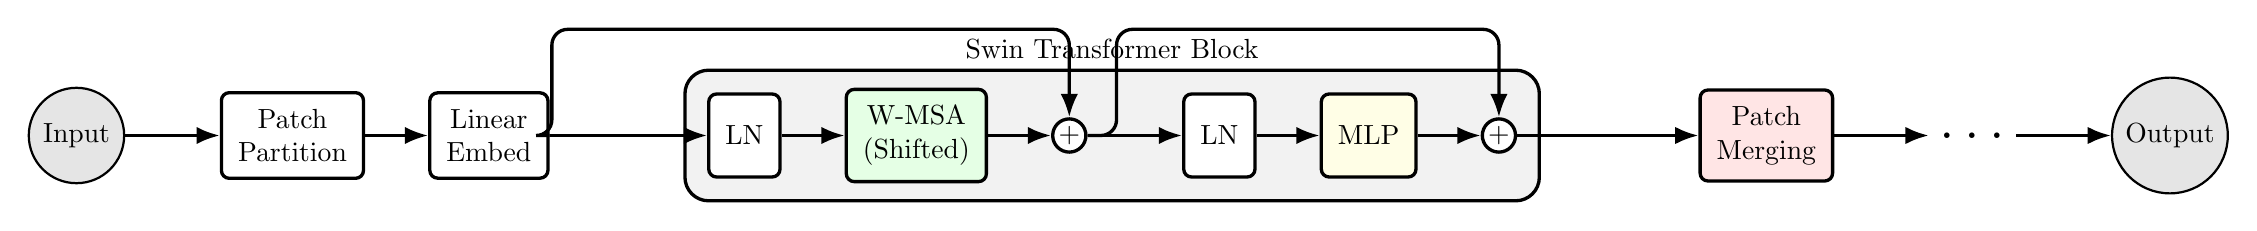
\begin{tikzpicture}[
    >=LaTeX, 
    very thick,
    node distance=1.0cm and 1.2cm,
    arrow/.style={
        ->,
        very thick,
        rounded corners=0.2cm
    },
    block/.style={
        rectangle,
        fill=gray!10,
        rounded corners=3mm,
        draw,
        very thick,
        inner sep=0.8em
    },
    layer/.style={
        rectangle,
        fill=white!10,
        rounded corners=1mm,
        inner xsep=0.6em,
        inner ysep=0.6em,
        minimum height=3.0em,
        align=center,
        draw,
        very thick
    },
    conv/.style={
        layer,
        fill=orange!10,
        draw=orange!80!black
    },
    relu/.style={
        layer,
        fill=yellow!10,
        draw=yellow!80!black,
        minimum height=2.5em
    },
    pool/.style={
        layer,
        fill=red!10,
        draw=red!80!black
    },
    input/.style={ 
        circle,
        minimum width=3.0em,
        draw,
        fill=gray!20,
        thick,
        align=center
    },
    sum/.style={
        circle,
        draw,
        fill=white,
        inner sep=0pt,
        minimum size=1.2em,
        node contents={+}
    }
]


    \node[input] (in) {Input};
    
    % Patch Partition
    \node[layer, right=of in] (embed) {Patch\\Partition};
    \draw[arrow] (in) -- (embed);
    
    \node[layer, right=0.8cm of embed] (lin) {Linear\\Embed};
    \draw[arrow] (embed) -- (lin);

    % Swin Block
    \node[layer, right=2.0cm of lin] (ln1) {LN};
    \node[layer, right=0.8cm of ln1, fill=green!10] (wmsa) {W-MSA\\(Shifted)};
    \node (sum1) [sum, right=0.8cm of wmsa];
    
    \node[layer, right=1.2cm of sum1] (ln2) {LN};
    \node[layer, right=0.8cm of ln2, fill=yellow!10] (mlp) {MLP};
    \node (sum2) [sum, right=0.8cm of mlp];

    \begin{scope}[on background layer]
        \node[block, fit=(ln1) (sum2), label=above:Swin Transformer Block] (swin_block) {};
    \end{scope}

    % Connections
    \draw[arrow] (lin) -- (ln1);
    \draw[arrow] (ln1) -- (wmsa);
    \draw[arrow] (wmsa) -- (sum1);
    \draw[arrow] (sum1) -- (ln2);
    \draw[arrow] (ln2) -- (mlp);
    \draw[arrow] (mlp) -- (sum2);

    % Skips
    \draw[arrow] (lin) -- ++(0.8,0) |- ($(ln1.north) + (0, 0.8)$) -| (sum1.north);
    \draw[arrow] (sum1) -- ++(0.6,0) |- ($(ln2.north) + (0, 0.8)$) -| (sum2.north);

    % Patch Merging
    \node[layer, right=2.0cm of swin_block, fill=red!10] (merge) {Patch\\Merging};
    \draw[arrow] (sum2) -- (merge);

    % Stages
    \node[right=1.2cm of merge] (dots) {\huge $\dots$};
    \draw[arrow] (merge) -- (dots);
    
    \node[input, right=of dots] (out) {Output};
    \draw[arrow] (dots) -- (out);

\end{tikzpicture}
\end{document}
